\section{Methodology}

\subsection{Problem Definition}
The market-making problem addressed in this work involves designing an optimal trading policy for an agent using reinforcement learning (RL). The agent aims to maximize profit while managing risks, particularly inventory risk. The market dynamics are modeled by the limit order book (LOB) and its dynamics, which define how the book evolves over time based on order flow and price movements. Our agent interacts with this environment by quoting bid and ask prices and adjusting offered quantities. As discussed previously, the main challenge for choosing an adequate agent and its policy lies in balancing profitability with risk management, especially regarding inventory at the close of the market, where overnight positions can expose the agent to significant risks.

\subsection{Formal Description of the RL Environment}
The RL environment is modeled as a continuous Markov chain. The state space is represented by variables that reflect the market's current conditions, including the Relative Strength Index (RSI), order imbalance, micro price, and price level distances for \(d\) levels in the order book. Formally, the state space can be written as:
$$
P(X_{t + \Delta t} \mid X_t) = P(X_{t + \Delta t} \mid X_{t}, X_{t - 1}, \dots, X_0).
$$
The evolution is continuous in time, meaning state changes occur at any point in continuous time, and the next event occurs after a sampled waiting time. The specific case in which the Markov Chain also has an associated reward distribution for each state transition is called a Markov Reward Process, and whenever the transitions are affected by some decision process it is called a Markov Decision Process, defined as a 4-tuple \( (S, A, P, R) \), where:

\begin{itemize}
	\item \( S \) is a set of states called the state space.
	\item \( A \) is a set of actions called the action space.
	\item \( P: S \times A \times S \to [0, 1] \) is the transition probability function defined as:
\end{itemize}

\begin{equation}
	P(r, s' | s, a) = \Pr(r_{t +1} = r, s_{t+1} = s' \mid s_t = s, a_t = a)
\end{equation}

for all \( s, s' \in S \), \( a \in A \) and $r \in \mathbb{R}$. This function gives the probability of transitioning to state \( s' \) from state \( s \) by taking action \( a \) and receiving the reward $r$ during this transition.

\begin{figure}[H]
	\centering
	\documentclass[tikz,border=10pt]{standalone}
\usepackage{pgf}
\usepackage{xcolor}

\begin{document}
	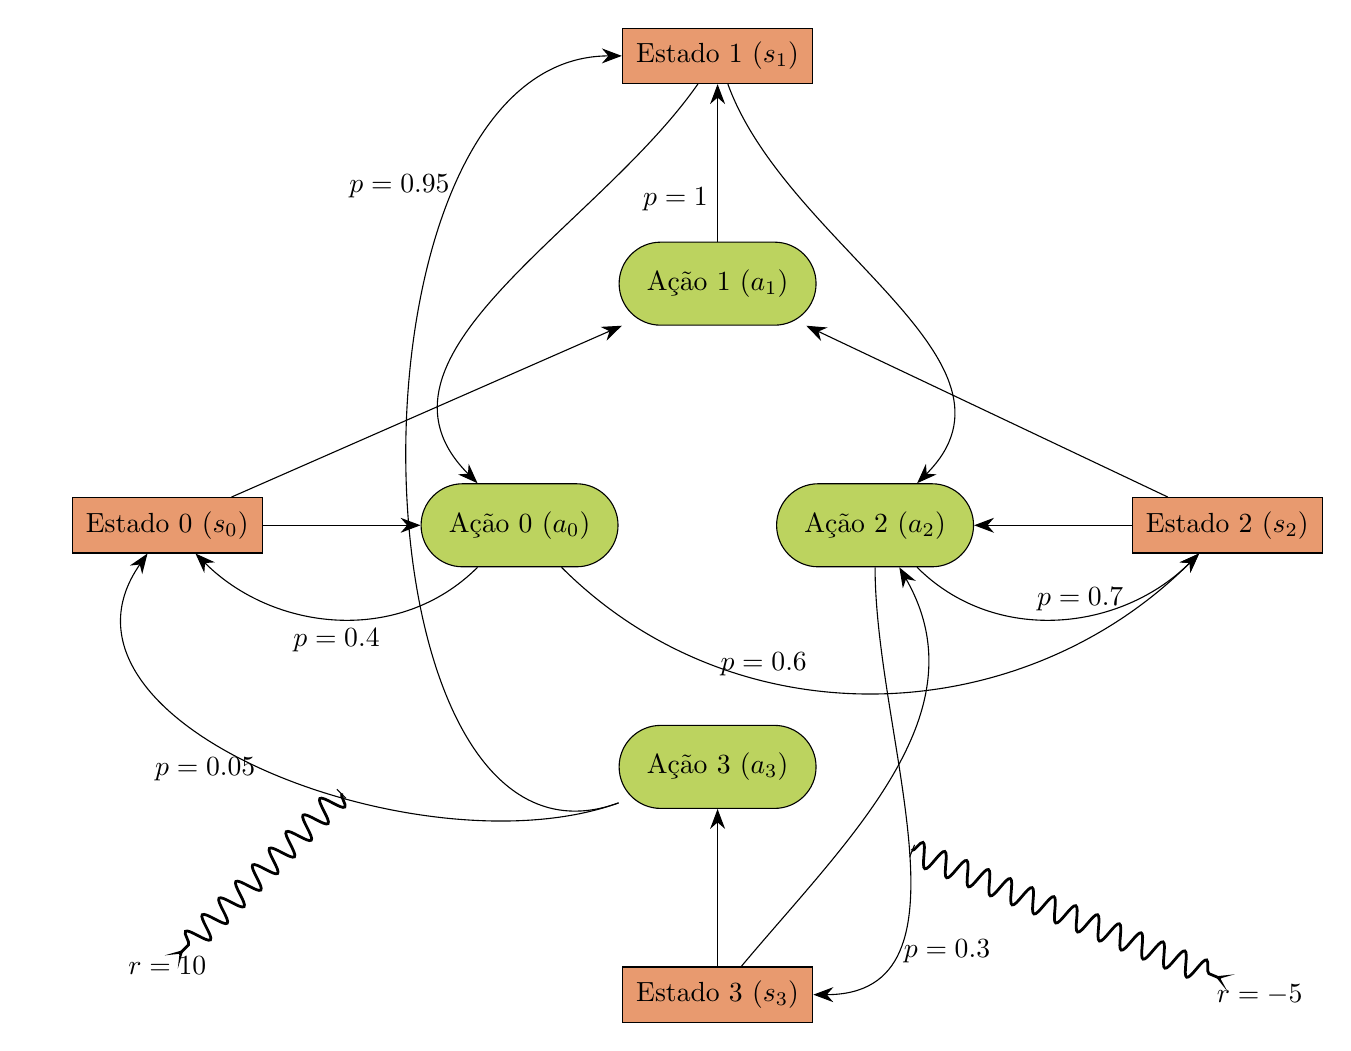
\begin{tikzpicture}
		\usetikzlibrary{arrows,automata,positioning,arrows.meta};
		\definecolor{statecolor}{HTML}{e89a6f};
		\definecolor{actioncolor}{HTML}{bcd35f};
		\tikzset{
			state/.style={
				shape=rectangle,
				draw=black,
				fill=statecolor,
				align=center,
				minimum height=2em,
				minimum width=4em,
				inner sep=5pt,
			},
			action/.style={
				shape=rectangle,
				draw=black,
				fill=actioncolor,
				align=center,
				inner sep=10pt,
				rounded corners=15pt,
			},
			reward/.style={
				|-,
				decoration={snake, amplitude=1.5mm, segment length=3mm},
				decorate,
				postaction={draw, line width=1pt, -{Stealth[scale=-0.8]}}
			},
			transition/.style={
				->,
				>={Stealth[scale=1.5]},
			}
		};
		\tikzset{node distance=2cm and 2cm}
    	\node[state] (s0) {Estado 0 ($s_0$)};

		\node[action, right=2cm of s0] (a0) {Ação 0 ($a_0$)};
		\node[action, above right=2cm and 0cm of a0] (a1) {Ação 1 ($a_1$)};
		\node[action, right=2cm of a0] (a2) {Ação 2 ($a_2$)};
		\node[action, below right=2cm and 0cm of a0] (a3) {Ação 3 ($a_3$)};

		\node[state, above=2cm of a1] (s1) {Estado 1 ($s_1$)};
		\node[state, right=2cm of a2] (s2) {Estado 2 ($s_2$)};
		\node[state, below=2cm of a3] (s3) {Estado 3 ($s_3$)};
		
		\node[draw=none, below right=2.8cm and 1cm of s0] (r0s) {};
		\node[draw=none, below=5cm of s0] (r0e) {$r=10$};
		
		\node[draw=none, above right=1.4cm and 1cm of s3] (r1s) {};
		\node[draw=none, right=5cm of s3] (r1e) {$r=-5$};
		
		\begin{scope} % actions
			\draw[transition] 
			(s0) 
			to
			(a0);
	
			\draw[transition] 
			(s0) 
			to
			(a1);
	
			\draw[transition] 
			(s1) 
			to[in=45, out=290]
			(a2);
	
			\draw[transition] 
			(s1) 
			to[in=135, out=235]
			(a0);
	
			\draw[transition] 
			(s2) 
			to
			(a1);
	
			\draw[transition] 
			(s2) 
			to
			(a2);
	
			\draw[transition] 
			(s3) 
			to
			(a3);
	
			\draw[transition] 
			(s3) 
			to[in=300, out=50]
			(a2);		
		\end{scope}
		
		\begin{scope} % transitions
			\draw[transition] 
			(a0)
			to[in=315, out=225] node[midway, below] 
			{$p = 0.4$} 
			(s0);
			
			\draw[transition] 
			(a0) 
			to[in=225, out=315] node[near start, right] 
			{$p = 0.6$} 
			(s2);
			
			\draw[transition] 
			(a1) 
			to[in=270, out=90] node[near start, left] 
			{$p = 1$} 
			(s1);
			
			\draw[transition] 
			(a2) 
			to[in=225, out=315] node[near end, left] 
			{$p = 0.7$} 
			(s2);
			
			\draw[transition] 
			(a2) 
			to[in=0, out=270] node[near end, right] 
			{$p = 0.3$} 
			(s3);
			
			\draw[transition] 
			(a3) 
			to[in=235, out=200] node[midway, left] 
			{$p = 0.05$} 
			(s0);
			
			\draw[transition] 
			(a3) 
			to[in=180, out=200] node[near end, left] 
			{$p = 0.95$} 
			(s1);
		\end{scope}
		
		\begin{scope}
			\draw[reward]
			(r0s)
			to
			(r0e);
			
			\draw[reward]
			(r1s)
			to
			(r1e);
			
		\end{scope}
	\end{tikzpicture}
\end{document}

	\caption{Discrete Markov Decision Process with 4 possible states and actions}
	\label{fig:mdp}
\end{figure}

\subsection{Description of the RL Environment}
The RL environment is modeled as a MDP, consisting of the state space \( \mathcal{S} \), action space \( \mathcal{A} \), reward function \( r \), and some transition dynamics, either known or unknown. 

For testing our framework of inserting restrictions for the Market Maker trader, our market simulation is modeled as follows:

\begin{itemize}
	\item \textbf{State Space:} Let \( \mathbf{S}_t \) denote the state of the environment at time \( t \). The state includes the relative strength index (RSI), order imbalance (OI), micro price \( P_{\text{micro}} \), and the price level distances \( \Delta P_i \) at \( d \) levels of the LOB:
	
	$$
	\mathbf{S}_t = \left( \text{RSI}_t, \text{OI}_t, P_{\text{micro},t}, \Delta P_{1,t}, \Delta P_{2,t}, \dots, \Delta P_{d,t} \right) \in \mathbb{R}^3 \times \mathbb{R}^{2d}.
	$$
	
	The components of the state space are defined as follows:
	
	- \textbf{Order Imbalance (OI):} Order imbalance measures the relative difference between buy and sell orders at a given time. It is defined as:
	$$
	\text{OI}_t = \frac{Q_t^{\text{bid}} - Q_t^{\text{ask}}}{Q_t^{\text{bid}} + Q_t^{\text{ask}}},
	$$
	where \( Q_t^{\text{bid}} \) and \( Q_t^{\text{ask}} \) represent the total bid and ask quantities at time \( t \), respectively. \( \text{OI}_t \in [-1, 1] \), with \( \text{OI}_t = 1 \) indicating complete dominance of bid orders, and \( \text{OI}_t = -1 \) indicating ask order dominance.
	
	- \textbf{Relative Strength Index (RSI):} The RSI is a momentum indicator that compares the magnitude of recent gains to recent losses to evaluate overbought or oversold conditions. It is given by:
	$$
	\text{RSI}_t = 100 - \frac{100}{1 + \frac{\text{Average Gain}}{\text{Average Loss}}},
	$$
	where the \textit{Average Gain} and \textit{Average Loss} are computed over a rolling window (commonly 14 periods). Gains are the price increases during that window, while losses are the price decreases.
	
	- \textbf{Micro Price (\( P_{\text{micro}} \)):} The micro price is a weighted average of the best bid and ask prices, weighted by their respective quantities:
	$$
	P_{\text{micro},t} = \frac{P_t^{\text{ask}} Q_t^{\text{bid}} + P_t^{\text{bid}} Q_t^{\text{ask}}}{Q_t^{\text{bid}} + Q_t^{\text{ask}}},
	$$
	where \( P_t^{\text{ask}} \) and \( P_t^{\text{bid}} \) represent the best ask and bid prices at time \( t \).
	
	\item \textbf{Action Space:} The action space \( \mathcal{A}_t \) represents the decisions made by the agent at time \( t \), including the bid and ask spreads \( \delta_t^{\text{ask}}, \delta_t^{\text{bid}} \) and the corresponding order quantities \( q_t^{\text{ask}}, q_t^{\text{bid}} \). Formally:
	$$
	\mathbf{A}_t = \left( \delta_t^{\text{ask}}, \delta_t^{\text{bid}}, q_t^{\text{ask}}, q_t^{\text{bid}} \right) \in \mathbb{R}^2 \times \mathbb{Z}^2.
	$$
	
	\item \textbf{Reward Function:} The reward function \( r_t \in \mathbb{R} \) reflects the agent's profit and inventory risk. It is based on the spread and executed quantities, as well as the inventory cost.
\end{itemize}

The agent interacts with the environment by choosing actions \( \mathbf{A}_t \) in response to observed states \( \mathbf{S}_t \), and the goal is to maximize cumulative rewards over time. The system's evolution follows a , and the transition probabilities between states depend on the agent's actions.

\subsection{Limit Order Book Evolution Dynamics}
The limit order book is modeled as a continuous-time Markov chain, where the timing of events follows a \textit{Hawkes process} to capture the clustering of order arrivals.

The Hawkes process is a \textit{self-exciting process}, where the intensity \( \lambda(t) \) depends on past events. Formally, the intensity \( \lambda(t) \) evolves as:
$$
\lambda(t) = \mu + \sum_{t_i < t} \phi(t - t_i),
$$
where \( \mu > 0 \) is the baseline intensity, and \( \phi(t - t_i) \) is the \textit{kernel function} that governs the decay of influence from past events \( t_i \). A common choice for \( \phi \) is an exponential decay:
$$
\phi(t - t_i) = \alpha e^{-\beta (t - t_i)},
$$
where \( \alpha \) controls the magnitude of the self-excitation and \( \beta \) controls the rate of decay.

The bid and ask prices are modeled by \textit{Ornstein-Uhlenbeck (OU) processes} to capture the mean-reversion behavior of spreads:
$$
ds_t = \theta(\mu - s_t) dt + \sigma dW_t,
$$
where \( s_t \) is the market spread at time \( t \), \( \theta \) is the rate of mean reversion, \( \mu_{spread} \) is the long-term spread mean and \( \sigma \) its volatility. The Wiener process \( W_t \) is used to represent random market fluctuations.

The bid and ask spreads \( \delta_t^{\text{bid}} \) and \( \delta_t^{\text{ask}} \) for orders conditioned on their arrival follow normal distributions:
$$
\delta_t^{\text{ask}} \sim \mathcal{N}(\mu + M_{t-1} + s_t, \sigma^2), \quad a_t^{\text{bid}} \sim \mathcal{N}(\mu + M_{t-1} - s_t, \sigma^2),
$$
where \( \mu_{\text{ask}} \) and \( \mu_{\text{bid}} \) are the respective means and \( \Delta a_t \) is the spread adjustment.

Whenever a new limit order that narrows the bid-ask spread or a market order arrive the mid-price is updated to reflect the top-of-book orders. The mid-price \( M \) at time $t+1$ is then obtained by averaging the maximum and minimum bid and ask prices in the book:

$$
M_{t+1} = \frac{2M_t + \delta^{ask}_{t} - \delta^{bid}_{t}}{2} 
\sim \mathcal{N}(\mu + M_{t}, \frac{\sigma^2}{2})
$$

The average of the best bid and ask prices therefore evolves according to a \textit{Brownian Motion} process:
$$
dM_t = \mu dt + \frac{\sigma^2}{2} dW_t,
$$
where \( W_t \) is a Wiener process.

The order quantities \( q_t^{\text{ask}} \) and \( q_t^{\text{bid}} \) are modeled as Poisson random variables:
$$
q_t^{\text{ask}}, q_t^{\text{bid}} \sim \text{Poisson}(\lambda_q),
$$
where \( \lambda_q \) is the average order size.

\subsection{Agent Objective}
The agent’s goal is to maximize its utility, which for our model is based on a Profit and Loss (PnL) score while still managing inventory risk. The choosen reward function is based on a risk-aversion enforced utility function, specifically the \textit{constant absolute risk aversion (CARA)}:
$$
R_t = U(\text{PnL}_t) = -e^{-\gamma \cdot \text{PnL}_t},
$$
where \( \gamma \) is the risk aversion parameter.

The PnL at time \( t \) is computed as:
$$
\text{PnL}_t = \delta_t^{\text{ask}} q_t^{\text{ask}} - \delta_t^{\text{bid}} q_t^{\text{bid}} + \text{I}_t \cdot \Delta M_t.
$$

The agent starting penalty for holding large inventory positions  is discounted from the \textit{PnL} score, as follows:
$$
\text{Penalty}_t = \eta \left( \text{Inventory}_t \cdot \Delta M_t \right)^+,
$$
$$
\text{PnL}_t := \text{PnL}_t - \text{Penalty}_t
$$
where \( \eta \) is the penalty factor applied to positive inventory changes.

The overall objective is to maximize cumulative utility while minimizing risk associated with inventory positions, and later insert restrictions so the risk for inventory is either limited at zero at market close, or incurring in larger penalties on the received rewards.